\documentclass{beamer}
\usetheme{Madrid}
\usepackage{hyperref}
\usepackage[utf8]{inputenc}
\usepackage[T1]{fontenc}
\usepackage{lmodern}
%\usepackage[mathscr]{euscript}
% \usepackage[usenames, dvipsnames]{xcolor}
\usepackage{mathtools}
\usepackage{amssymb}
\usepackage{amsthm}
%\usepackage{xparse}
\usepackage{xspace}
\usepackage{tikz-cd}
\usepackage{adjustbox}

% \numberwithin{equation}{section}
\usepackage[utf8]{inputenc}
\usepackage[T1]{fontenc}
\usepackage{lmodern}
%\usepackage[mathscr]{euscript}
\usepackage[margin=1.33in]{geometry}
% \usepackage{setspace}
\setstretch{1.125}
\usepackage[usenames, dvipsnames]{xcolor}
% \usepackage{graphicx}
\usepackage{mathtools}
\usepackage{amssymb}
\usepackage{amsthm}
%\usepackage{xparse}
\usepackage{xspace}
\usepackage{tikz-cd}
\usepackage[backref=page, bookmarks=false]{hyperref}
% \usepackage[capitalize, noabbrev]{cleveref}
\setcounter{tocdepth}{1}

\newcommand{\mb}{\mathbf}

\newcommand{\iso}{\cong}
\newcommand{\isoto}{\xrightarrow{\simeq}}

\newcommand{\Z}{\mathbb Z}
\newcommand{\Q}{\mathbb Q}
\newcommand{\R}{\mathbb R}
\newcommand{\C}{\mathbb C}
\newcommand{\T}{\mathbb T}
\newcommand{\F}{F}
\newcommand{\ii}{\mathbf i}
\newcommand{\mcal}[1]{\mathcal{#1}}

\newcommand{\op}{\mathsf{op}}
\newcommand{\GL}{\mathrm{GL}}
\newcommand{\PSL}{\mathrm{PSL}}
% \newcommand{\Diff}{\mathrm{Diff}}
\newcommand{\Lie}{\mathrm{Lie}}
\newcommand{\Zn}{\Z(n)}
\newcommand{\Rn}{\R(n)}
\newcommand{\Bdot}{B_\bullet}
\newcommand{\Edot}{E_\bullet}
\newcommand{\BdotG}{B_\bullet G}
\newcommand{\EdotG}{E_{\bullet}G}
\newcommand{\BdotH}{B_\bullet H}
\newcommand{\BnablaG}{B_\nabla G}
\newcommand{\EnablaG}{E_\nabla G}
\newcommand{\BdotGamma}{B_\bullet \Gamma}
\newcommand{\GFG}{\Gamma \backslash F / G}
\newcommand{\GFR}{\Gamma \backslash F / \R}
\newcommand{\GF}{\Gamma \backslash F}
\newcommand{\Diff}{\mathrm{Diff}^+(S^1)}
\newcommand{\Mfld}{Mfld}
\newcommand{\Witt}{\mathfrak{w}}
\newcommand{\LieVir}{\mathfrak{vir}}
% \newcommand{\FGG}(F/G}

\newcommand{\point}{\ast}

\newcommand{\Zf}{\mb{Z}_2^F}
\newsavebox{\pullback}
\sbox\pullback{%
\begin{tikzpicture}%
\draw (0,0) -- (1ex,0ex);%
\draw (1ex,0ex) -- (1ex,1ex);%
\end{tikzpicture}}

\DeclareMathOperator{\Ext}{Ext}
\DeclareMathOperator{\Hom}{Hom}

\newtheorem{lemma}[equation]{Lemma}
\newtheorem{corollary}[equation]{Corollary}
\newtheorem{proposition}[equation]{Proposition}
\newtheorem{thm}[equation]{Theorem}
\newtheorem{theorem}[equation]{Theorem}
\newtheorem*{mainthm}{\cref{main_thm}}

\theoremstyle{definition}
\newtheorem{example}[equation]{Example}
\newtheorem{definition}[equation]{Definition}
\newtheorem{claim}[equation]{Claim}
\newtheorem{conj}[equation]{Conjecture}
\newtheorem{question}[equation]{Question}

\theoremstyle{remark}
\newtheorem{remark}[equation]{Remark}
\newtheorem*{fct}{Fact}
\newtheorem*{note}{Note}


\crefname{thm}{Theorem}{Theorems}
\crefname{lem}{Lemma}{Lemmas}
\crefname{cor}{Corollary}{Corollaries}
\crefname{prop}{Proposition}{Propositions}
\crefname{ex}{Exercise}{Exercises}
\crefname{exm}{Example}{Examples}
\crefname{defn}{Definition}{Definitions}
\crefname{claim}{Claim}{Claims}
\crefname{rem}{Remark}{Remarks}
\crefname{fct}{Fact}{Facts}
\crefname{note}{Note}{Notes}

\newcommand{\term}{\emph} % e.g. "The \term{trace} is defined to be..."

\DeclarePairedDelimiter\abs{\lvert}{\rvert}
\DeclarePairedDelimiter\set{\{}{\}}
\DeclarePairedDelimiter\paren{(}{)}
\DeclarePairedDelimiter\ang{\langle}{\rangle}
\DeclarePairedDelimiter\ket{\lvert}{\rangle}

\makeatletter
	\let\oldparen\paren
	\def\paren{\@ifstar{\oldparen}{\oldparen*}}
\makeatother

\usepackage{microtype}
\usepackage{hypcap}

\hypersetup{
 colorlinks,
 linkcolor={red!50!black},
 citecolor={green!50!black},
 urlcolor={blue!80!black}
}

% make cleveref use the Oxford comma:
% see https://tex.stackexchange.com/questions/161338
\newcommand{\creflastconjunction}{, and\nobreakspace}

\newcommand{\TODO}{\textcolor{red}{TODO}}

\newcommand{\cat}{\mathsf}
\newcommand{\Man}{\cat{Man}}
\newcommand{\Sh}{\cat{Sh}}
\newcommand{\Ch}{\cat{Ch}}
\newcommand{\sSet}{\cat{sSet}}

\newcommand{\Hsm}{H_{\mathrm{SM}}}

\newcommand{\Sym}{\mathrm{Sym}}
\newcommand{\fg}{\mathfrak g}
\newcommand{\gl}{\mathfrak{gl}}
\newcommand{\tr}{\mathrm{tr}}
\newcommand{\OmegaR}{\Omega^1 \otimes i\R}
\newcommand{\chern}{(c_1)^\nabla}


\renewcommand{\d}{\mathrm d}
\newcommand{\ud}{\,\d}

\newcommand{\tGam}{\widetilde\Gamma}
\newcommand{\CExt}{\mathrm{CExt}}
\newcommand{\Map}{\mathrm{Map}}

% was this deifned somewhere else...?
\newcommand{\AlgVir}{\mathfrak{vir}}
\newcommand{\GpVir}{\widetilde\Gamma}

% maintenance
\newcommand{\CW}[1]{\footnote{\textcolor[rgb]{0.60,0.00,0.50}{CW: #1}}}%
\newcommand{\AD}[1]{\footnote{\textcolor[rgb]{0.00,0.50,0.50}{AD: #1}}}%
\newcommand{\YL}[1]{\footnote{\color{orange} {\bf YL:} {#1}}}

\newcommand{\IZ}{I\mb{Z}}
% \newcommand{\Diff}{\mathrm{Diff}^+(S^1)}


\AtBeginSection[]
{
  \begin{frame}
    \frametitle{Table of Contents}
    \tableofcontents[currentsection]
  \end{frame}
}

\newcommand{\mb}{\mathbf}
\newcommand{\Mfld}{Mfld}
\newcommand{\iso}{\cong}
\newcommand{\isoto}{\xrightarrow{\simeq}}

\newcommand{\Z}{\mathbb Z}
\newcommand{\Q}{\mathbb Q}
\newcommand{\R}{\mathbb R}
\newcommand{\C}{\mathbb C}
\newcommand{\T}{\mathbb T}
\newcommand{\F}{F}
\newcommand{\ii}{\mathbf i}


\newcommand{\op}{\mathsf{op}}
\newcommand{\GL}{\mathrm{GL}}
\newcommand{\PSL}{\mathrm{PSL}}
% \newcommand{\Diff}{\mathrm{Diff}}
\newcommand{\Lie}{\mathrm{Lie}}
\newcommand{\Zn}{\Z(n)}
\newcommand{\Rn}{\R(n)}
\newcommand{\Bdot}{B_\bullet}
\newcommand{\Edot}{E_\bullet}
\newcommand{\BdotG}{B_\bullet G}
\newcommand{\EdotG}{E_{\bullet}G}
\newcommand{\BdotH}{B_\bullet H}
\newcommand{\BnablaG}{B_\nabla G}
\newcommand{\EnablaG}{E_\nabla G}
% \newcommand{\BdotGamma}{B_\bullet \Gamma}
\newcommand{\GFG}{\Gamma \backslash F / G}
\newcommand{\GFR}{\Gamma \backslash F / \R}
\newcommand{\GF}{\Gamma \backslash F}
\newcommand{\Diff}{\mathrm{Diff}^+(S^1)}
% \newcommand{\Mfld}{Mfld}
\newcommand{\Witt}{\mathfrak{w}}
\newcommand{\LieVir}{\mathfrak{vir}}
% \newcommand{\FGG}(F/G}

\newcommand{\point}{\ast}
\renewcommand{\d}{\mathrm d}
\newcommand{\ud}{\,\d}
\newcommand{\tGam}{\widetilde\Gamma}
\newcommand{\CExt}{\mathrm{CExt}}
\newcommand{\Map}{\mathrm{Map}}

\newcommand{\Vir}{\mathrm{Vir}}





\newcommand{\term}{\emph} % e.g. "The \term{trace} is defined to be..."



\usepackage{microtype}
\usepackage{hypcap}

\hypersetup{
 colorlinks,
 linkcolor={red!50!black},
 citecolor={green!50!black},
 urlcolor={blue!80!black}
}

% make cleveref use the Oxford comma:
% see https://tex.stackexchange.com/questions/161338
\newcommand{\creflastconjunction}{, and\nobreakspace}

\newcommand{\TODO}{\textcolor{red}{TODO}}

\newcommand{\cat}{\mathsf}
\newcommand{\Man}{\cat{Man}}
\newcommand{\Sh}{\cat{Sh}}
\newcommand{\Ch}{\cat{Ch}}
\newcommand{\sSet}{\cat{sSet}}

\newcommand{\Hsm}{H_{\mathrm{SM}}}

\newcommand{\Sym}{\mathrm{Sym}}
\newcommand{\fg}{\mathfrak g}
\newcommand{\gl}{\mathfrak{gl}}
\newcommand{\tr}{\mathrm{tr}}
\newcommand{\OmegaR}{\Omega^1 \otimes i\R}
\newcommand{\chern}{(c_1)^\nabla}

\newtheorem{prop}[equation]{Proposition}


%Information to be included in the title page:
\title{Differential Cohomology and Virasoro Central Extensions}
\author[Yu Leon Liu ]{Yu Leon Liu} % auteur
\institute[Rouen University]{\textbf {Rouen University}}\institute{Harvard University}
\date[April 2rd 2022] {April 3rd 2022 \\ \vspace{5mm} Based on [\href{https://arxiv.org/abs/2112.10837}{arXiv:2112.10837}] \\ Joint with Arun Debray and Christoph Weis}
\titlegraphic{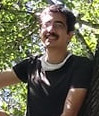
\includegraphics[width=.2\textwidth,height=.2\textheight]{tree.jpg}
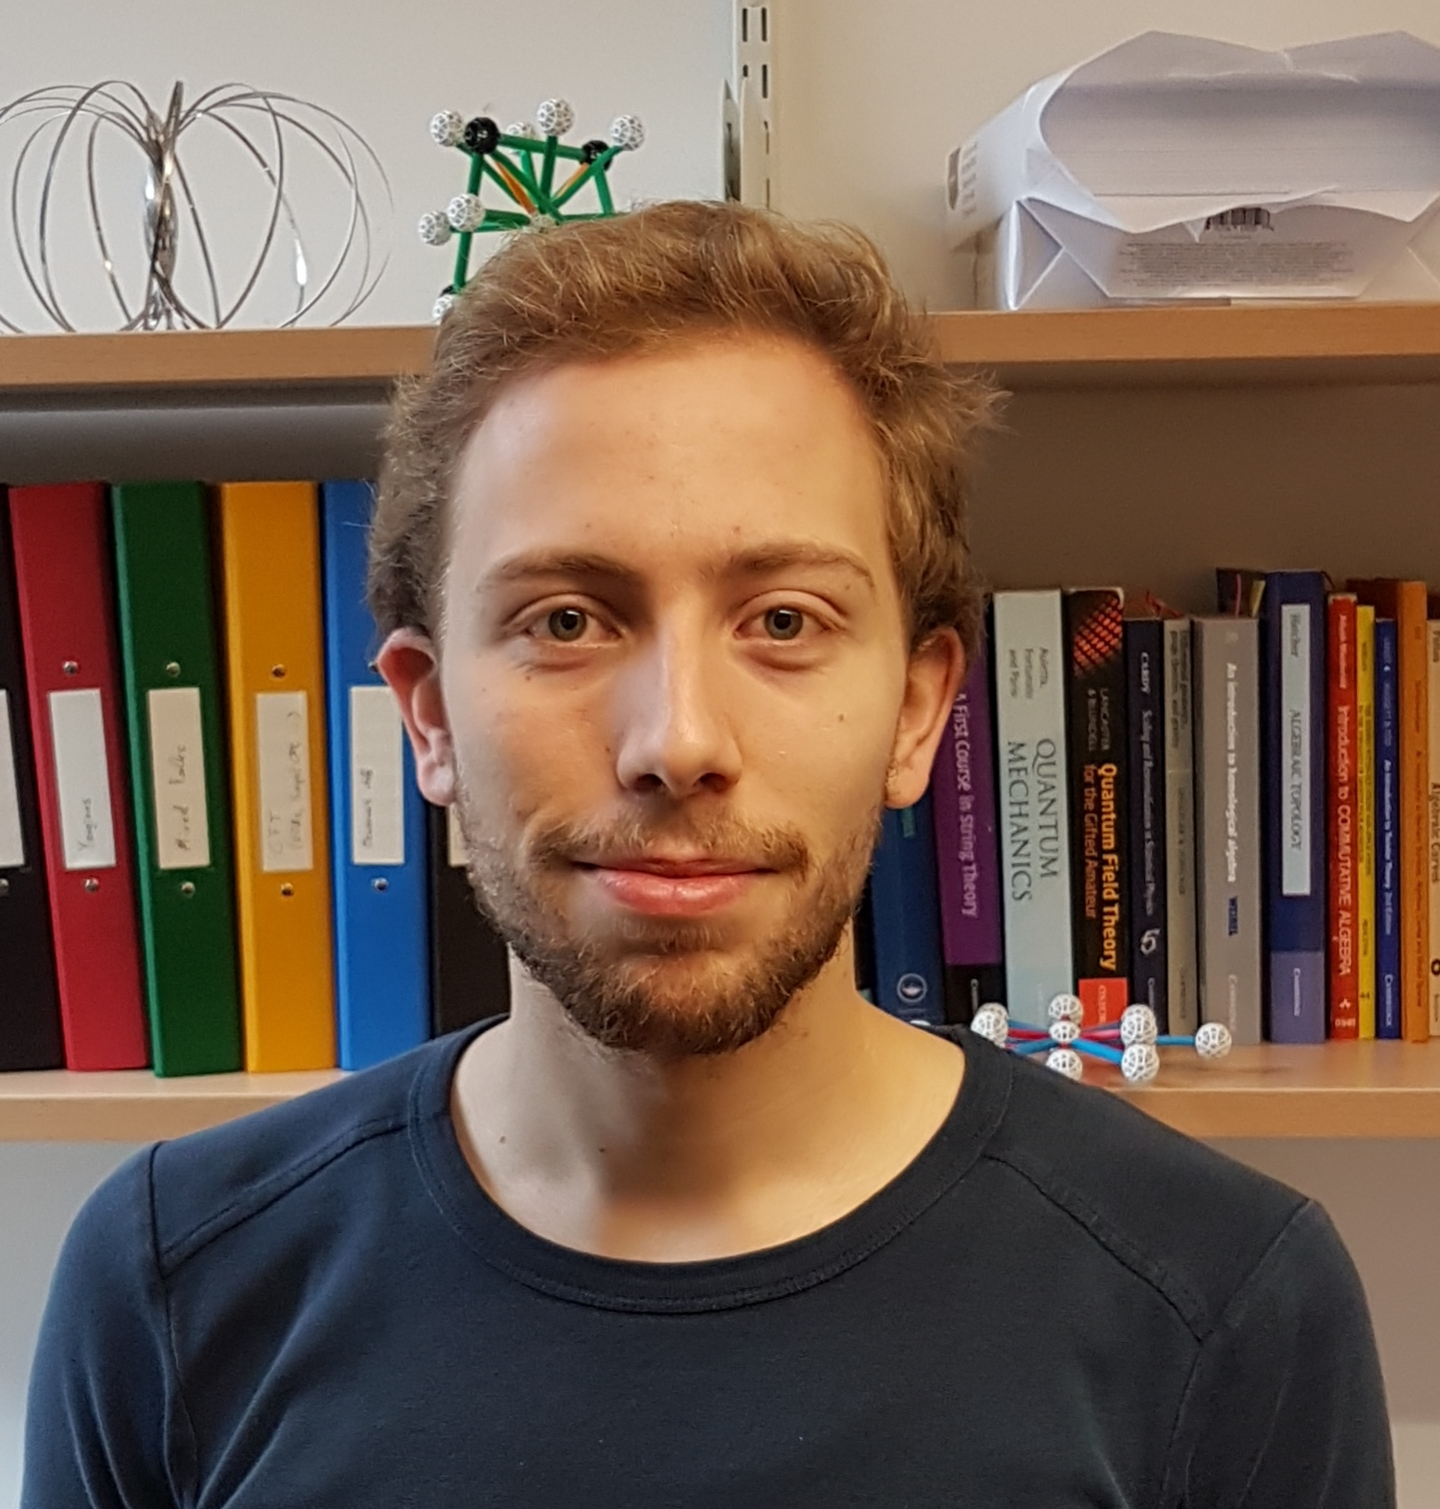
\includegraphics[width=.2\textwidth,height=.2\textheight]{me.jpg}
}

\begin{document}

\frame{\titlepage}

% toc
\begin{frame}
    \frametitle{Table of Contents}
    \tableofcontents
    \end{frame}


\section{Motivation}
\begin{frame}
\frametitle{Motivation}
\begin{itemize}
    \item <1 -> The \alert{Virasoro groups} describe space-time symmetries 
    of 2d CFTs. As such, it is important to physics (string theory, condensed matter) and 
    mathematics (geometric representation theory).
    \item <2 -> \alert{Virasoro groups} is a $\mb{R}$ family of central extension of $\Diff$, the group of 
    orientation preserving smooth automorphism of $S^1$. 
    \item <3 -> The central extension is describe by the 
    \alert{Bott-Thurston cocyle}. 
    \item <4 -> The goal of this talk is to give a novel geometric description 
    these central extensions, using differential cohomology, affirmativaly answering a conjecture of Freed-Hopkins.
\end{itemize}

\end{frame}

\section{Virasoro groups and central extensions}

\begin{frame}
    \frametitle{Bott-Thurston cocycles}

Recall that $\Diff$ is the group of orientation preserving smooth automorphism of $S^1$. 
It is an infinite-dimensional Frechet Lie group. \pause
    \begin{definition}
The Virasoro group $\Vir_\lambda$, for $\lambda \in \mb{R}$, is a $U(1)$ central extension of $\Diff$, described by the \alert{Bott-Thurston cocycle}
$B_\lambda: \Diff \times \Diff \to U(1)$: \pause
\begin{equation}
    B_\lambda(\gamma_1, \gamma_2) = \exp\left(-\frac{i\lambda}{48\pi}\int_{S^1} \log(\gamma_1'
        \circ\gamma_2) \ud(\log(\gamma_2))'\right)
\end{equation}
for $\gamma_1, \gamma_2 \in \Diff$, viewed as morphisms $S^1 \to S^1$.
\end{definition}
\end{frame}

\begin{frame}
    \frametitle{Central Extensions}
    Let's briefly review what is a central extension: \pause
    \begin{definition}
        Let $G$ be a group and $A$ be an abelian group, a central extension of $G$
        by $A$ is a group $\tilde{G}$ with short exact sequence:
        \begin{eqnarray}
            0 \to A \to \tilde{G} \to G \to 1
        \end{eqnarray}
        such that subgroup $A \subset \tilde{G}$ is in the center, that is, 
        it commutes with every element of $\tilde{G}$.
    \end{definition}
\end{frame}

\begin{frame}
    \frametitle{Central extension as group cohomology: I}
    As many other things, central extensions can be classified by cohomology groups: \pause 
    
    \begin{prop}
        Let $G$ be a discrete group, then the isomorphism class of central extensions of $G$ by $A$ is 
        classified by group cohomology class $H^2(G; A) \simeq H^2(BG; A)$, where $BG$ is the 
        classifying space of $G$.
    \end{prop}\pause

    Given a cocycle class $b \in C^2(G;A)$, viewed as a map $b : G \times G \to A$ 
    satisying some cocycle conditions. Then $\tilde{G} = G \times A$ as a set, with multiplication 
    $(g, a) \cdot (g', a') \coloneqq (g \cdot g', a + a' + b(g, g'))$. \pause \\
    The map $\tilde{G} \to G$ is  $(g, a) \mapsto g$.
\end{frame}

\begin{frame}
    \frametitle{Central extension as group cohomology: II}
    \alert{Problem}:  Smooth $U(1)$ central extensions of nondiscret Lie groups are \alert{NOT} classified 
    by ordinary cohomology classes. \pause \vspace{5mm}

    We need a cohomology theory that remembers the smooth structures. \pause 

    \vspace{5mm} The answer is \alert{differential cohomology}.
\end{frame}


\section{Differential cohomology}

\begin{frame}
    \frametitle{Sheaves on smooth manifolds}
    Let $M$ be a manifold, then the ordinary cohomology groups  $H^*(M; A)$ depends 
    only on the homotopy classes of $M$. It is the cohomology of the constant sheave 
    $\underline{A}$ on $M$.
    On the other hand, the $i$-th differential form on $M$, $\Omega^i(M)$ is sensitive 
    to the smooth structure of $M$. \pause \vspace{5mm}
    
    We can view both constant sheaves and 
    differential forms as sheaves on $\Mfld$, the site of smooth manifolds. \pause 

    \vspace{5mm}
    Even though $\Omega^i$ are not homotopy invariant, the chain complex of sheaves 
    $\Omega^* = 0 \to \Omega^0 \xrightarrow{d} \Omega^1 \xrightarrow{d} \dots$ is a homotopy invariant,
    in fact,
    \begin{theorem}[de Rham]
        The chain complex $\Omega^*$ is the constant sheave $\underline{\R}$, as a chain complex concentrated in degree 0.
    \end{theorem}
\end{frame}

\begin{frame}
    \frametitle{Sheaves $\Z(n)$}
    With this in mind, we define the (chain complex of) sheave $\Z(n)$ as 
    \begin{equation}
        \Z(n) = \underline{\Z} \to \Omega^0 \to \Omega^1 \to \dots \to \Omega^{n-1} \to 0.
    \end{equation} \pause 
    These sheaves $\Z(n)$ are both sensitive to topology (from $\Z$) and the smooth 
    structure (from $\Omega^i$). \pause \vspace{5mm}

    There is also a form of integration.  let $M$ be a closed oriented $d$-dimensional 
    manifold, then there is an integration map:
    \begin{equation}
        \int_M: H^*(M; \Z(n)) \to H^{*-d}(*; \Z(n-d)).
    \end{equation}
    There is also a relative version of this.
\end{frame}

\begin{frame}
    \frametitle{Example: $\Z(1)$ and line bundles}
    A cocycle in $C^2(M; \Z(1))$ can be describe as follows:
    fix an open covering $\{U_i\}$ of $M$, we have $0$-form ($\R$-valued functions) $a$ on 
    the open subsets $U_{ij} = U_i \cap U_j$, and $\Z$-valued functions $f_{ijk}$ on intersections $U_{ijk}$, such that 
    $a_{ij} - a_{jk} + a_{ik} = f_{ijk}.$\pause \vspace{5mm}

    This precisely describe the data of a $U(1)$ principal bundle on $M$!
    \begin{prop}
        $H^2(M; \Z(1))$ is the group of isomorphism classes of $U(1)$ principal bundles on $M$.
    \end{prop}

    Furthermore, $H^2(M; \Z(2))$ is the group of isomorpism classes of $U(1)$ principal bundles with connections on $M$ 
    (Hint: for the cocycle here we need also $1$-form $\alpha_i$ on $U_i$, with $\alpha_i - \alpha_j = d a_{ij}$).
\end{frame}

\begin{frame}
    \frametitle{$\Z(1)$ and central extensions}
    While $H^2(-; \Z(1))$ classifies $U(1)$ principal bundle, $H^3(-; \Z(1))$ classifies 
    $U(1)$ central extensions: \pause

    \begin{theorem}
        Let $G$ be a smooth (possibly infinite dimensional) Lie group, $\BdotG$ 
        its classifying space. Then 
        $H^3(BG; \Z(1))$ classifies smooth central extensions of $G$ by $U(1)$.
    \end{theorem} \pause 

    $\BdotG$ is the classifying space of $G$, viewed as a sheave on $Mfld$.

\end{frame}

\begin{frame}
    \frametitle{Differential characteristic classes}
    Let $G$ be a Lie group, and $\Bdot G$ the classifying space. Then $H^*(\Bdot G; \underline{\Z})$ 
    are the characteristic classes of $G$. Similiarly, $H^*(\Bdot G; \Z(n))$ are differential 
    characetristic classes of $G$. \pause \vspace{5mm}

    We will  need the following key fact:
    \begin{theorem}[Bott, Freed-Hopkins]
        $H^4(\Bdot\GL_1^+(\R); \Z(2)) \simeq \R$.
    \end{theorem} \pause \vspace{5mm}

    They are the differential first Pontryagin classes.
\end{frame}


\section{Main theorem}
\begin{frame}
    \frametitle{Key Idea I}
    We want to get a $\R$ family of central extension of $\Diff$ by $U(1)$, therefore 
    we want a $\R$ family in $H^3(\Bdot\Diff, \Z(1))$. We get this by pullback and integration: \pause 

    \vspace{5mm} 
    Consider the canonical $\Diff$ action on $S^1$, note that \pause
    \begin{itemize}
        \item <1 -> The quotient $S^1/\Diff$ has a map to $\Bdot\Diff = * /\Diff$.
        Since the action of $\Diff$ on $S^1$ is orientation preserving, this is a oriented 
        $S^1$ fiber bundle. \pause
        \item <2 -> The tangent bundle of $S^1$ gives a map $TS^1: S^1 \to \Bdot\GL^+_1(\R)$. Since
        the action of $\Diff$ on $S^1$ is smooth, the tangent bundle is $\Diff$-equivariant. Equivalently,
        the tangent bundle factors through the quotient as a map $TS^1: S^1/\Diff \to \Bdot \GL^+_1(\R)$.
    \end{itemize}
\end{frame}

\begin{frame}[fragile]
    \frametitle{Key Idea II}
    To summarize, we have a span of maps:
    \begin{equation}
        %\label{eqn:transgression_space_diagram}
        \begin{tikzcd}
        S^1/\Diff \arrow[r, "TS^1"] \arrow[d]
        & \Bdot\GL^+_1(\R) \\
        \Bdot\Diff.
        & 
        \end{tikzcd}
        \end{equation}
    Note the vertical map is a $S^1$ fibration, something we can integrate against. 

    Therefore we get a map:
    \begin{equation}
        %\label{eqn:transgression_space_diagram}
        \begin{tikzcd}
        H^4(S^1/\Diff; \Z(2))  \arrow[d, "\int_{S^1}"]
        & H^4(\Bdot \GL^+_1(\R); \Z(2)) \arrow[l]\\
        H^3(\Bdot\Diff; \Z(1)).
        & 
        \end{tikzcd}
        \end{equation} 
\end{frame}

\begin{frame}
    \frametitle{Main theorem}
    Finally, we can state the conjecture of Freed and Hopkins that we proved: \vspace{5mm}
    \begin{theorem}[Y.L., Arun Debray, Christoph Weis]
        The image of map $\R \simeq H^4(\Bdot \GL^+_1(\R); \Z(2)) \to H^3(\Bdot\Diff; \Z(1))$
        are the Virasoro central extensions $\Vir_\lambda$.
    \end{theorem}

    \vspace{5mm} Furthermore, we explicitly recovers the Bott-Thurston cocylces when calculating the 
    map on cocycles.
\end{frame}

\begin{frame}
    \frametitle{Proof sketch I}
    We construct explicit cocycles and compute the map on the 
    level of cocycles.
    \begin{itemize}
        \item <1 -> We find $1$-form cocycles for $H^4(\Bdot \GL^+_1(\R); \Z(2))$, 
        using the canonical simplicial resolution of $\Bdot \GL^+_1(\R)$.
        \item <2 -> We pullback to  $1$-form cocycles on $S^1/\Diff$, using the simplicial 
        realization of $S^1 = Fr_+(S^1)/\GL^+_1(\R)$, where $Fr_+(S^1)$ is the oriented frame bundle.
    \end{itemize}
\end{frame}

\begin{frame}[fragile]
    \frametitle{Proof sketch II}
    Here's the key point of the proof:
    \begin{itemize}
        \item <1 -> Now we move the cocycles across the double complex associated to the 
        bisimplicial object $S^1/\Diff = \GL^+_1(\R) \backslash Fr_+(S^1) / \GL^+_1(\R)$, to get 
        cocycles on the simplicial resolution for $S^1/\Diff$.
        \begin{adjustbox}{max totalsize={.7\textwidth}{.5\textheight},center}
            \begin{tikzpicture}
                \draw  node (N20) at (-6,0) {$\Omega^1(\Gamma^{\times 2} \times F)$}
                       node (N10) at (-3,0) {$\Omega^1(\Gamma \times F)$}
                       node (N11) at (-3,3) {$\Omega^1(\Gamma \times F \times \R)$}
                       node (N01) at (0,3)  {$\Omega^1(F \times \R)$}
                       node (N02) at (0,6)  {$\Omega^1(F \times \R^{\times 2})$};
                \draw [->] (N10) -- (N20);
                \draw [->] (N10) -- (N11);
                \draw [->] (N01) -- (N11);
                \draw [->] (N01) -- (N02);
                \begin{scope}[shift={(1,-0.5)}]
                    \draw  node (C20) at (-6,0) {$x_2 \d x_1$} 
                           node (C10) at (-3,0) {$x\ \ud\log(v)$}
                           node (C11) at (-3,3) 
                           [align=center]{\\
                           $\textcolor{blue}{x \log \gamma^\prime} -$ \\
                           $\textcolor{red}{x \log \gamma^\prime} = 0$}
                           node (C01) at (0,3)  {$\log(v)\ \ud\log(\gamma^\prime)$}
                           node (C02) at (0,6)  {\hspace{5em}
                           $-\log(\gamma_1'\circ\gamma_2) \ud\log(\gamma_2)$};
                    \draw [|->] (C10) -- (C20);
                    \draw [|->,draw=red] (C10) -- (C11);
                    \draw [|->,draw=blue] (C01) -- (C11);
                    \draw [|->] (C01) -- (C02);
                \end{scope}
            \end{tikzpicture}
        \end{adjustbox}
            % \item <2 -> We integrate over $S^1$ and recovers the Bott-Thurston cocyle.
    \end{itemize}
\end{frame}

\begin{frame}
    \frametitle{Proof sketch III}
    \begin{itemize}
        \item <1 -> Lastly, we integrate over $S^1$ and immediately see that 
        we recover the Bott-Thurston cocycles! Q.E.D.
    \end{itemize}
\end{frame}

\begin{frame}
    \frametitle{Last slide}
    \huge Thank you for listening!
\end{frame}
% As such they have applications to 
% \begin{itemize}
%     \item<1 -> String theory. 2d CFT is the language to describe string worldsheet.
%     \item<2 -> Geometric reprensentation theory. 2d CFT is closely related to reprensentation
%     of affine Kacs-Moody groups/algebras and geometric Langlands.
%     \item<3 -> Condensed matter physics.  Theories like Wess-Zumino-Wess models many important 
%     condensed matter sysmtems like (fraction) Quantum Halls.
%     \item<4 -> Algebraic Geometry of surfaces. 
% \end{itemize}


% table of contents


\end{document}
